\documentclass[10pt,letterpaper]{article}
\usepackage{geometry}
\geometry{letterpaper, portrait, margin=0.5in}
\usepackage[utf8]{inputenc}
\usepackage{amsmath}
\usepackage{amsfonts}
\usepackage{amssymb}
\usepackage{graphicx}
\usepackage{subcaption}
\usepackage{array}
\usepackage{hyperref}
\usepackage{adjustbox,lipsum}
\usepackage{gensymb}
\setlength{\parindent}{0pt}
\renewcommand\refname{Related documents/articles to read:}

\begin{document}
\title{\scshape\LARGE University of Waterloo \vfill \huge\bfseries KMOS Work Documentation \vfill}
\author{Robert Burnet \\ rcburnet@uwaterloo.ca \\ 20465122 }
\maketitle

\newpage

\tableofcontents

\listoffigures

\listoftables

\newpage

\section{Introduction and Related Documents/Articles}

This is a document describing what I did over the term in regards to the SAMI and ALFALFA surveys. Similar to a journal except more formal. All my work and scripts can be found on my github page: github.com/rcburnet/S16work .
\begin{thebibliography}{1}
\bibitem{github}My github page for all my scripts: \url{github.com/rcburnet/S16work}. Master branch is all the work I did on the desktop workstation. Also see laptop branch for all the work I did on my laptop.
\bibitem{SAMI instrument front-page}SAMI instrument front-page: \url{http://sami-survey.org/}\\
\bibitem{SAMI Early Data Release}SAMI Early Data Release (this is the data used): \url{http://sami-survey.org/edr}\\
\bibitem{ALFALFA front-page} ALFALFA front-page: \url{http://egg.astro.cornell.edu/alfalfa/}\\
\bibitem{K98}K98 (SFR from Halpha relation) article: \url{http://www.annualreviews.org/doi/pdf/10.1146/annurev.astro.36.1.189}\\
\bibitem{sensitivity} Completeness, Sensitivity, and Detection limits of ALFALFA survey article: Haynes et al. 2011 \url{https://arxiv.org/pdf/1109.0027v1.pdf}\\
\bibitem{alfalfa data} ALFALFA data: \url{http://egg.astro.cornell.edu/alfalfa/data/}\\
\bibitem{mass function} ALFALFA Science Goals: Giovanelli et al. 2005 \url{http://iopscience.iop.org/article/10.1086/497431/pdf}\\
\bibitem{sersic}Sersic Profile article: Graham and Driver 2005 \url{https://arxiv.org/pdf/astro-ph/0503176v1.pdf}\\

\end{thebibliography}
All the work I'd done with SAMI and ALFALFA were carried out on my laptop. I've ported my work to the desktop in the directory /home/rcburnet/S16work/ . The scripts that were developed and used on my laptop may not work on the desktop without changing directory designations in the scripts. The main difference in the directory designation (and most likely the only difference) is the user (eg. /home/rburnet/... is the designation on my laptop, where as /home/rcburnet/... is the designation on the desktop). I've put all the data I manipulated/created/worked with/etc on my laptop using the laptop scripts onto the desktop workstation in the directory /home/rcburnet/SAMI. The directory $\sim$ from here on will refer to the desktop directory /home/rcburnet/ . The following sections detail what I did for this project. It describes and explains the various scripts I developed, showing their outputs as figures. For a more detailed description of each of the scripts, read through their comments and the Documentation text files in their directories. This document is intended to work as a brief overview of everything.\\


\section{Sources' Description}
\label{sec:sources}
There are in total 107 SAMI targets in the Early Data Release (EDR) (see the SAMI website \cite{SAMI instrument front-page}). The EDR datacubes are already calibrated and reduced. They can be downloaded from the SAMI website. Of those, 65 were found within the ALFALFA survey area of 7074 deg$^2$. The ALFALFA survey area spans 7.5h R.A. to 16.5h R.A. ("spring" region) and 22h R.A. to 3h R.A. ("fall" region) and 0\degree Dec. to 36\degree Dec. \cite{mass function}. Of the 65 within the ALFALFA survey area, 7 have corresponding HI detections in the ALFALFA survey (see a.70 catalog in \cite{alfalfa data}). All 65 targets are listed below by their GAMA IDs. The targets with ALFALFA names and which are in bold are the 7 that have corresponding HI detections. To see specific details of each target, see the SAMI-EDR data table \cite{SAMI Early Data Release} which tabulates their GAMA IDs as well as relevant physical features, also see the ALFALFA a.70 catalog \cite{alfalfa data}. \\

\begin{table}[h!]
\caption{Source Description} \label{tab: source}
\noindent\adjustbox{max width=\textwidth, max height=4in}{%
\begin{tabular}{|l|l|}
\hline
\textbf{GAMA ID} & \textbf{ALFALFA ID} \\ \hline
386268 & \\
345820 & \\
517164 & \\
417486 & \\
517205 & \\
422639 & \\
381215 & \\
517302 & \\
381229 & \\
417568 & \\
422683 & \\
417580 & \\
209181 & \\
599582 & \\
599689 & \\
599761 & \\
599838 & \\
599877 & \\
279818 & \\
302846 & \\
279891 & \\
623620 & \\
377962 & \\
373173 & \\
\textbf{623641} & \textbf{193636}\\
279886 & \\
279878 & \\
373202 & \\
623679 & \\
218717 & \\
\textbf{279917} & \textbf{198516}\\
218713 & \\
373248 & \\
325390 & \\
\textbf{623726} & \textbf{193643}\\
279943 & \\
623712 & \\
302994 & \\
623722 & \\
\textbf{216843} & \textbf{193647}\\
373284 & \\
288992 & \\
230714 & \\
272831 & \\
289089 & \\
220320 & \\
230776 & \\
289116 & \\
289185 & \\
230829 & \\
220383 & \\
\textbf{220371} & \textbf{223261}\\
289200 & \\
617945 & \\
617989 & \\
\textbf{91924} & \textbf{715963}\\
91963 & \\
77710 & \\
618143 & \\
91999 & \\
618152 & \\
\textbf{79635} & \textbf{243769}\\ \hline
\end{tabular}}
\end{table}

\newpage
The following sections deal with the above 65 targets and their relevant info found in the SAMI-EDR and ALFALFA a.70 catalog. You can download the SAMI data cubes (specifically red cubes) from the SAMI data page. The cubes are on the desktop in $\sim$/SAMI/data/ .

\newpage
\section{Work}
\subsection{July 4: Getting Started}
Spent most of my time understanding the SAMI and ALFALFA data. The SAMI data from the EDR are already reduced and calibrated, so unlike my work with KMOS, no further calibration was needed. I would start first by reading through the relevant papers on the SAMI website \cite{SAMI instrument front-page}, as well as any relevant ALFALFA papers on the ALFALFA website \cite{ALFALFA front-page}, especially anything to do with the data and instruments themselves. Read through the articles/pages in the above introduction section. You can also look through anything in the bookmarks.html bookmark file in $\sim$/S16work/bookmarks.html), although it won't be necessary.\\

After reading through the relevant papers/articles on SAMI and ALFALFA - after getting familiar with the data and instruments - you should download the SAMI data of the 65 targets that you will be working with. You can download the SAMI data right from the SAMI website. ALFALFA a.70 catalog which details the sources with HI detections can be found on the ALFALFA survey website.

\subsection{July 11 - July 22: Creating H$\alpha$ and continuum images}
After I familiarized myself with SAMI and ALFALFA (the data and insturments), I found 7 SAMI targets that had HI detections in the ALFALFA survey by comparing the coordinates of the two catalogs and finding targets which aligned (see /home/rburnet/S16work/SAMI/pair$\_$sami$\_$alfalfa.py). I created a script ($\sim$/S16work/SAMI/collapse$\_$cube$\_$Halpha$\_$complete.py) to collapse the cubes of the 7 SAMI sources with HI detections in the ALFALFA a.70 catalog between the FWHM of the H$\alpha$ profile of each target, as well as plot their spectrum between the two NII lines. Another script \\($\sim$/S16work/SAMI/collapse$\_$cube$\_$Halpha$\_$complete$\_$without$\_$HI$\_$detections.py) collapses the cubes of the 58 other targets that are within the ALFALFA survey area but don't have corresponding HI detections between the FWHM of their H$\alpha$ profiles. The following figure \ref{fig: 91924 Halpha image} is an example of the output image of target 91924 and figure \ref{fig: 91924 Spectrum} it's spectrum plot. Note: the dark blue curve is the total flux, light blue line is half maximum of H$\alpha$ profile, red line is mean continuum flux, and the two vertical lines designate the spectral extent of the FWHM (the spectral range of the collapsed H$\alpha$ image). To see the other H$\alpha$ images of the 7 SAMI targets with HI detections, see $\sim$/S16work/SAMI/Halpha$\_$images/ .

\begin{figure}[h!]
\center
\caption{91924 H$\alpha$ image}\label{fig: 91924 Halpha image}
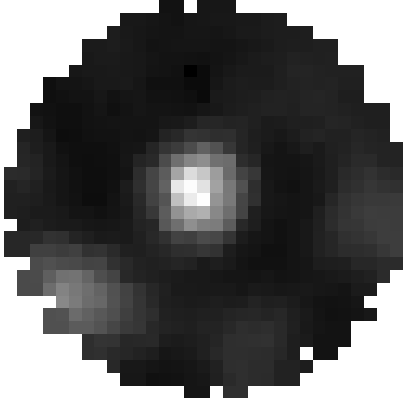
\includegraphics[scale=0.4]{figures/91924_Halpha_image.png}
\end{figure}

\begin{figure}[h!]
\center
\caption{91924 Spectrum}\label{fig: 91924 Spectrum}
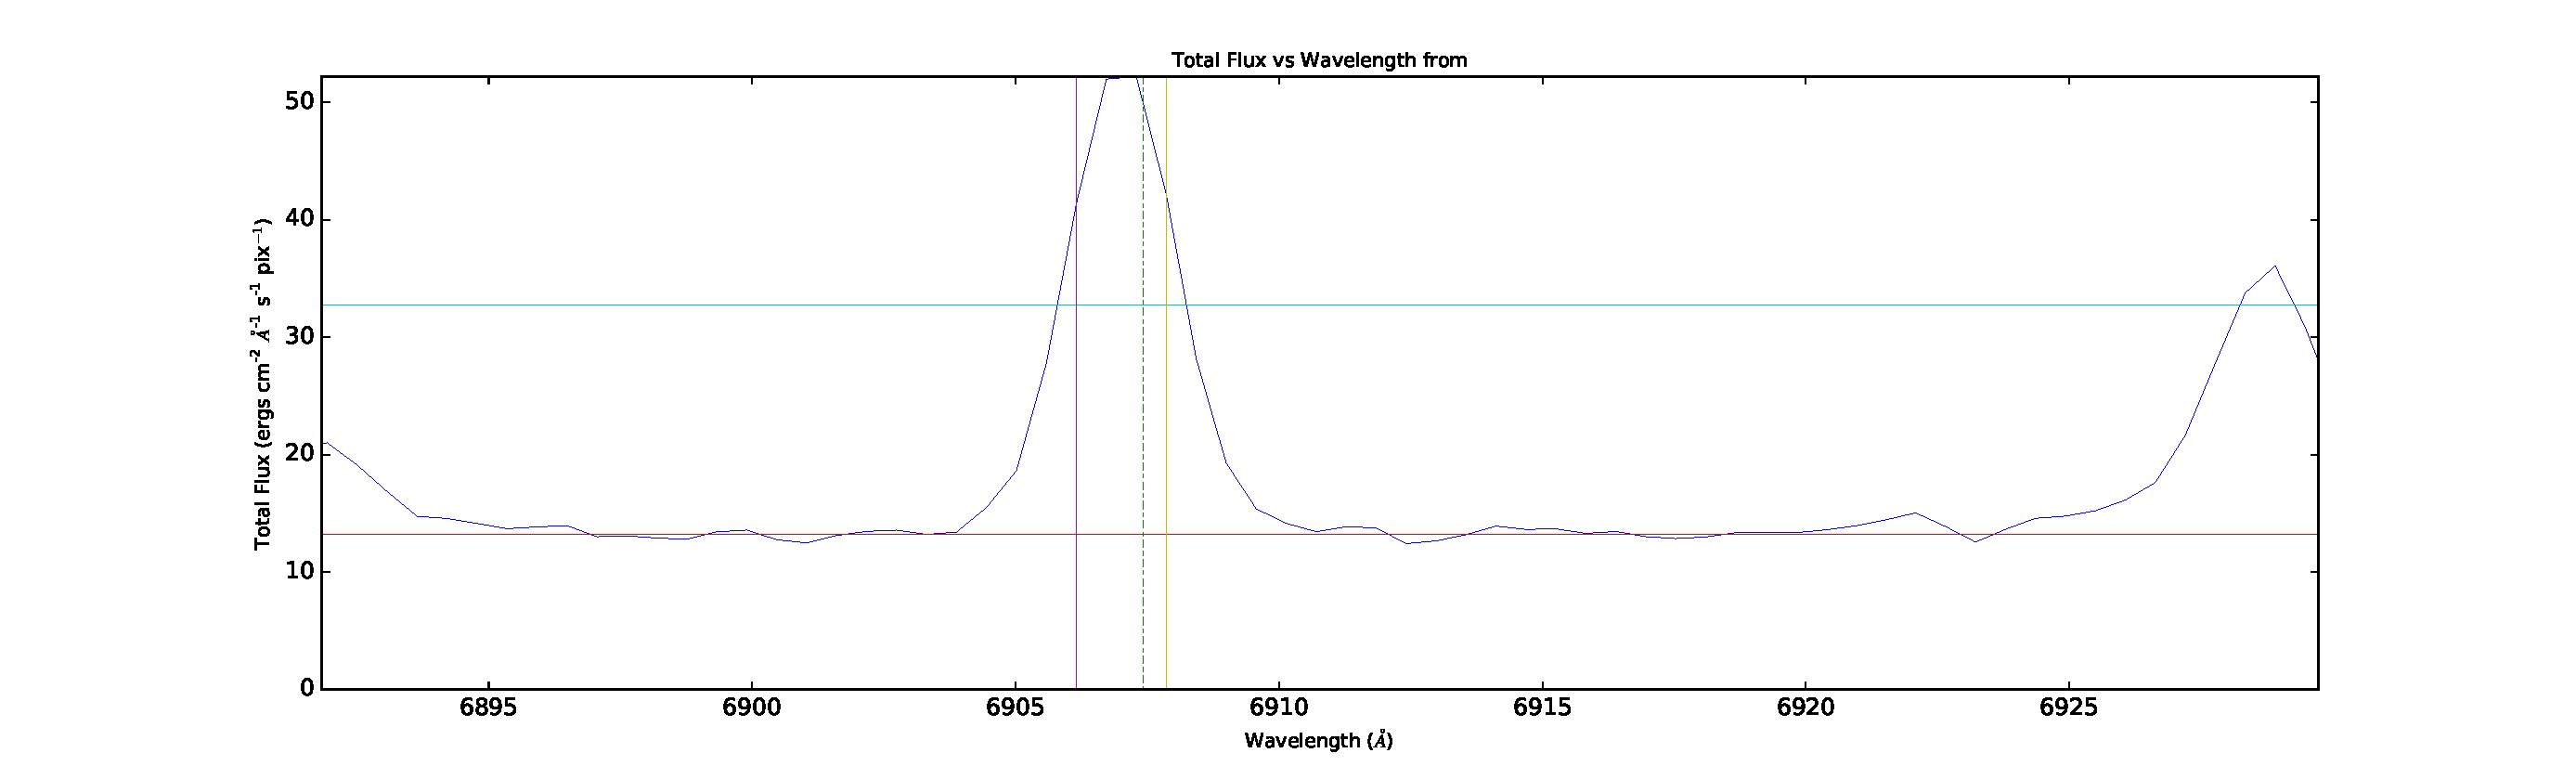
\includegraphics[scale=0.4]{figures/91924_red_7_Y13SAR1_P014_15T029fitscollapsed.pdf}
\end{figure}

\newpage

Another script ($\sim$/S16work/SAMI/collapse$\_$cube$\_$continuum$\_$complete.py) collapses the cubes of the 7 SAMI targets with HI detections between the H$\alpha$ and second NII lines (outside of their profile) to effectively create images of the local continuum of those cubes. The following figure \ref{fig: 91924 continuum image} is an example of the output continuum image of target 91924. To see the other continuum images of the 7 SAMI targets with HI detections, see $\sim$/S16work/SAMI/continuum$\_$images/ .

\begin{figure}[h!]
\center
\caption{91924 continuum image}\label{fig: 91924 continuum image}
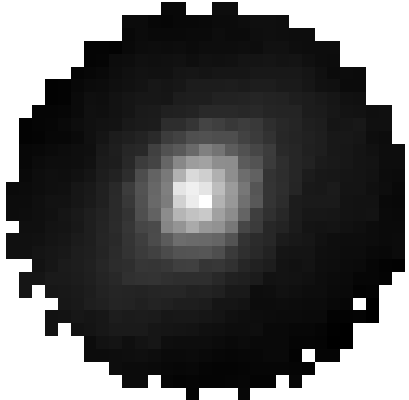
\includegraphics[scale=0.4]{figures/91924_continuum_image.png}
\end{figure}

\subsection{July 25 - August 12: Converting HI flux to HI gas mass, converting H$\alpha$ flux to SFR, calculating SFR/HI gas mass ratios, plotting SFR/HI gas mass vs M$_{star}$ and SFR vs HI gas mass}
Next, I created a script ($\sim$/S16work/SAMI/Halpha$\_$to$\_$SFR/Halpha$\_$to$\_$SFR.py) that converts H$\alpha$ flux to SFR of the 7 SAMI targets that have HI detections using the K98 H$\alpha$ luminosity to SFR relation \cite{K98}, as well as generates SFR maps as fits files. Using those SFR maps, I created a script ($\sim$/S16work/SAMI/Halpha$\_$to$\_$SFR/SFR$\_$HI$\_$gas$\_$mass$\_$ratio.py) which takes the total integrated SFR from each of the 7 targets' SFR maps as well as their reported HI gas masses in the ALFALFA a.70 catalog and prints their ratios to terminal. The SFR maps look the same as the Halpha images, just with units in M$\odot$/yr/pc$^2$.\\

I did something similar for the other 58 targets. However, since these targets had no HI detections, I had to use the 50\% completeness limit of the survey as a detection limit \cite{sensitivity} to calculate upper limits to the HI gas mass of these targets. I created a script ($\sim$/S16work/SAMI/HI$\_$gas$\_$mass$\_$upper$\_$limits/HI$\_$gas$\_$mass$\_$upper$\_$limits$\_$using$\_$50$\_$percent$\_$completeness$\_$limit.py) which uses that detection limit to calculate the upper limits to the HI gas mass of the 58 targets and writes them to a text file ($\sim$/S16work/SAMI/HI$\_$gas$\_$mass$\_$upper$\_$limits/HI$\_$gas$\_$mass$\_$upper$\_$limits$\_$using$\_$50$\_$percent$\_$completeness$\_$limit.txt).\\

23 of the targets had no detectable H$\alpha$, so I had to calculate as well an upper limit to the H$\alpha$ flux (and thus to the SFRs) of these targets using a 3$\sigma$ detection limit (see the following script for further details). I created a script \\($\sim$/S16work/SAMI/Halpha$\_$to$\_$SFR/Halpha$\_$to$\_$SFR$\_$and$\_$SFR$\_$to$\_$HI$\_$gas$\_$mass$\_$ratio$\_$no$\_$HI$\_$detections.py) which calculates the upper limits to the HI gas mass of the 58 targets, as well as the total integrated SFR for targets which have detectable H$\alpha$ and upper limits to the SFRs for the 23 targets which don't have detectable H$\alpha$, and prints the ratios of the SFR/HI gas masses to terminal. \\

I created a script ($\sim$/S16work/SAMI/Halpha$\_$to$\_$SFR/SFR$\_$plots.py) which uses the output of the above scripts to create two plots: 1) SFR/HI gas mass vs M$_{star}$ and 2) SFR vs HI gas mass. They are both split into 3 data groups: 1) The 7 SAMI targets with HI detections and detectable H$\alpha$ (actual SFRs and HI gas masses calculated), 2) The 35 targets with no HI detections but detectable H$\alpha$ (actual SFRs, upper limits to HI gas masses calculated), and 3)The 23 targets with no HI detections and no detectable H$\alpha$ (upper limits to both SFRs and HI gas masses calculated). The two plots are shown below in figures \ref{fig: SFR/HI gas mass vs Mstar} and \ref{fig: SFR vs HI gas mass}.\\

\begin{figure}[h!]
\center
\caption{SFR/HI gas mass vs M$_{star}$}\label{fig: SFR/HI gas mass vs Mstar}
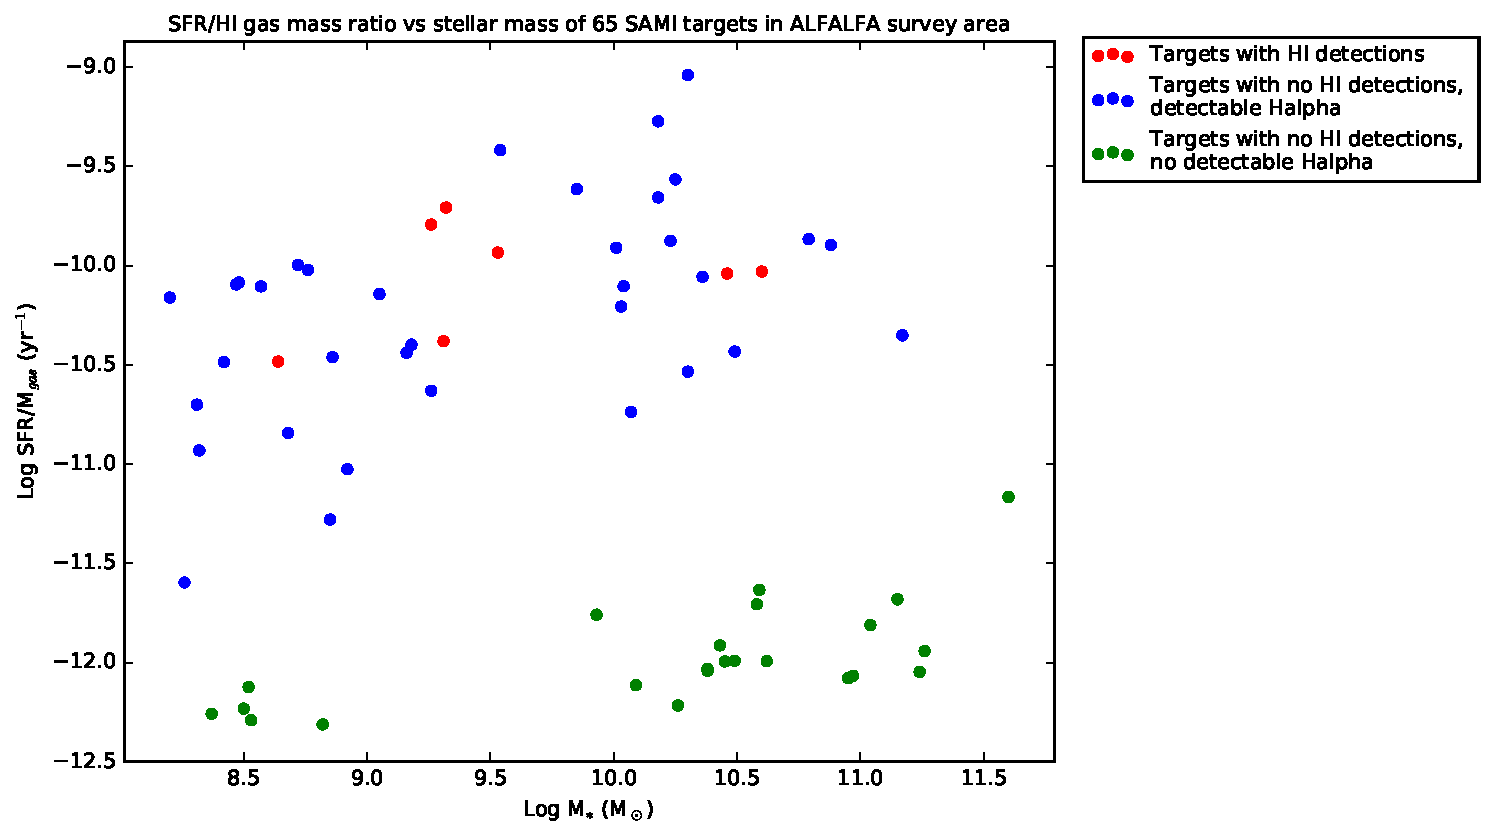
\includegraphics[scale=0.4]{figures/SFR_HI_gas_mass_ratio_vs_Mstar.pdf}
\end{figure}

\begin{figure}[h!]
\center
\caption{SFR vs HI gas mass}\label{fig: SFR vs HI gas mass}
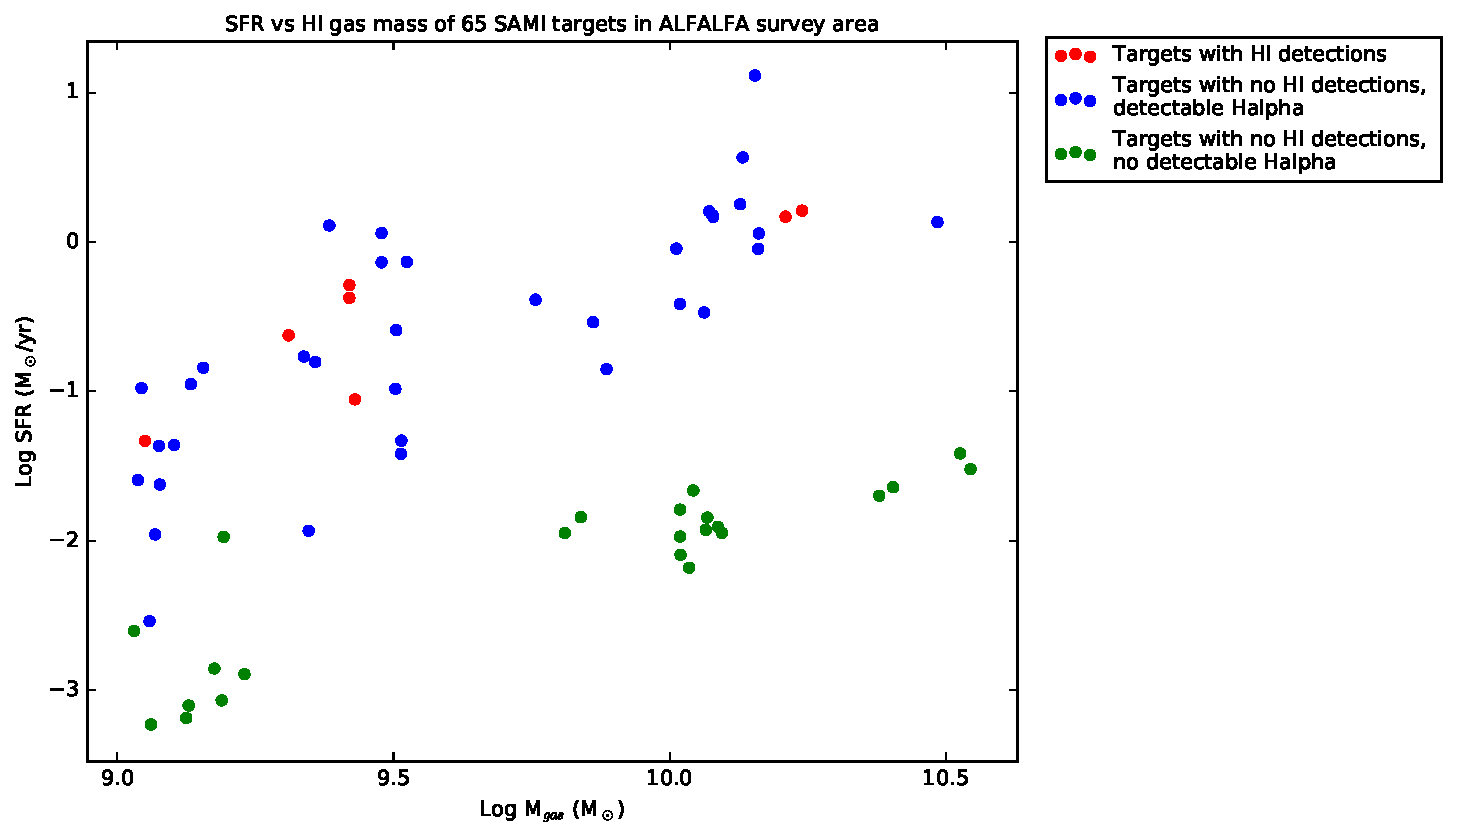
\includegraphics[scale=0.4]{figures/SFR_vs_HI_gas_mass.pdf}
\end{figure}

\subsection{August 15: Attempt at Sersic Profile fit, documentation}
I attempted to fit a Sersic profile (for details on the Sersic model, see Graham and Driver 2005 \cite{sersic}) to the radial profiles of the targets (I(R) vs R plots of H$\alpha$ maps). Unfortunately I did not have enough time to complete it. I began work in the directory $\sim$/S16work/SAMI/effective$\_$radius/ . The idea was to fit a Sersic profile to the radial profiles, and extrapolate from the model to retrieve the effective radii of the targets in H$\alpha$. The effective radii of the continuum of the targets are reported in the SAMI EDR catalog. We had planned to analyse the morphology of the H$\alpha$ distribution against the HI gas distribution, but did not get to it. I had trouble trying to fit the Sersic profile as I was convolving the PSF the wrong way.\\

The script $\sim$/S16work/SAMI/effective$\_$radius/radial$\_$profile.py may be useful as it plots the radial profiles of the 65 SAMI targets and saves them to $\sim$/S16work/SAMI/effective$\_$radius/figures/ . The radial profile of 91924 is given below as an example in figure \ref{fig: 91924 Radial profile}. Note: the blue curve is the radial profile plotted, the green line is the I$_e$ (intensity at R$_e$ given I(0), incorrect value as my method was wrong). I thought I could use the plotted I$_e$ to find R$_e$ (as the point of intersection of the line and radial profile would designate the effective radius), however how I applied the Sersic model was wrong.\\

\begin{figure}[h!]
\center
\caption{91924 Radial Profile}\label{fig: 91924 Radial profile}
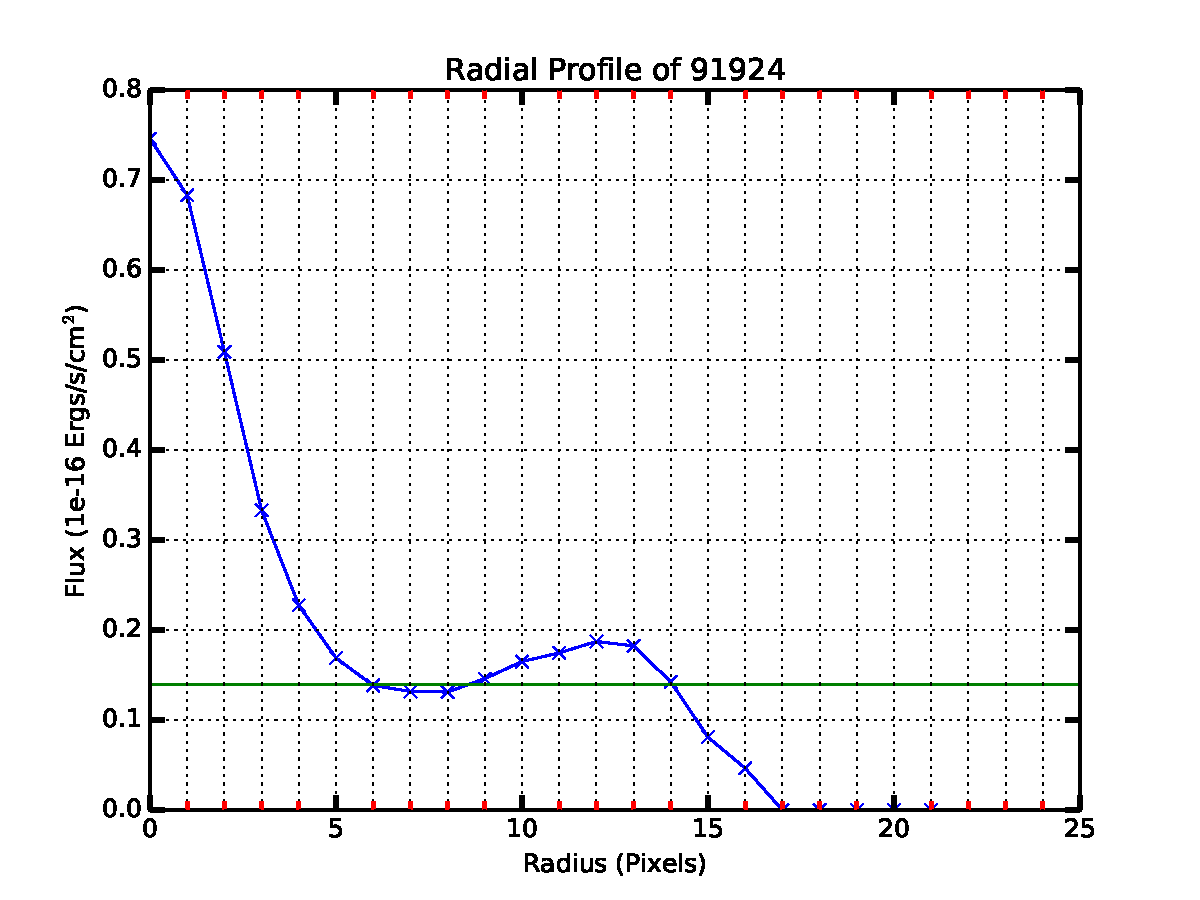
\includegraphics[scale=0.4]{figures/91924_radial_profile.pdf}
\end{figure}

\newpage

Originally, I was convolving the data with the PSF and fitting a Sersic model to it. However, we instead want to convolve the model and fit it to the data (ideally with a $\chi^2$ test) to get the right parameters. The parameters for the Sersic model are the R$_e$ (effective radius, the radius at which half the total light of the galaxy is within), I$_0$ (central intensity), and n (Sersic index). I was having trouble convolving the PSF with the model and decided to begin document my work instead.\\


\newpage

\end{document}